\documentclass[12pt,french]{article}

%___________________________
%===    Configurations 12.09.2013
%------------------------------------------------------
%packages permettant d'augmenter le nombre de registres de dimension et donc d'éviter les erreurs de compilation dûs aux packages tikz, pstricks and compagnie
\usepackage{etex}
%___________________________
%===    Pour le français
%------------------------------------------------------
\usepackage[utf8x]{inputenc}
\usepackage[T1]{fontenc}
\usepackage{babel}
\FrenchFootnotes

%___________________________
%===    Polices d'écriture
%------------------------------------------------------
%\usepackage{mathpazo}
\usepackage{frcursive} % Pour l'écriture cursive
\usepackage[upright]{fourier}% l'option permet d'avoir les majuscules droites dans les formules mathématiques
\usepackage[scaled=0.875]{helvet}

%___________________________
%===    Les couleurs
%------------------------------------------------------
\usepackage[dvipsnames,table]{xcolor}
%
\newcommand{\rouge}[1]{{\color{red} #1}}
\definecolor{midblue}{rgb}{0.145,0.490,0.882}
\newcommand\MaCouleur{midblue}

%___________________________
%===   Redéfinition des marges par défaut
%------------------------------------------------------
\setlength\paperheight{297mm}
\setlength\paperwidth{210mm}
\setlength{\evensidemargin}{0cm}% Marge gauche sur pages paires
\setlength{\oddsidemargin}{0cm}%{-0.5cm}% Marge gauche sur pages impaires
\setlength{\topmargin}{-2cm}% Marge en haut
\setlength{\headsep}{0.5cm}% Entre le haut de page et le texte
\setlength{\headheight}{0.7cm}% Haut de page
\setlength{\textheight}{25.2cm}% Hauteur de la zone de texte
\setlength{\textwidth}{17cm}% Largeur de la zone de texte

\usepackage{lscape} %permet le format paysage du document
\usepackage{xspace} % création automatique d'espaces dans les commandes
\setlength{\parindent}{0pt}

\usepackage{fancyhdr}
\pagestyle{fancy}
%
\renewcommand{\headrulewidth}{0pt}% pas de trait en entête
\newcommand\RegleEntete[1][0.4pt]{\renewcommand{\headrulewidth}{#1}}%commande pour ajouter un trait horizontal en entête

\newcommand{\entete}[3]{\lhead{#1} \chead{#2} \rhead{#3}}
\newcommand{\pieddepage}[3]{\lfoot{#1} \cfoot{#2} \rfoot{#3}}
%
%\renewcommand{\chaptermark}[1]{\markboth{#1}{}} % enregistre le titre courant du chapitre
    %en-tete droite page [paire] et {impaire}
%\rhead[]{\textbf{\leftmark.}}
    %en-tete gauche page [paire] et {impaire}
%\lhead[\textbf{\chaptername~\thechapter.}]{}


\usepackage{enumerate} %permet la modif de la numérotation et de poursuivre une numérotation en cours avec \begin{enumerate}[resume]
\usepackage{enumitem}
\frenchbsetup{StandardLists=true}%frenchb ne s'occupera pas des listes
\setenumerate[1]{font=\bfseries,label=\arabic*\degres)} % numérotation 1°) 2°) ...
%\setenumerate[2]{font=\itshape,label=(\alph*)} % sous-numérotation (a) (b) ...
\setenumerate[2]{font=\bfseries,label=(\alph*)} % sous-numérotation (a) (b) ...

\usepackage{lastpage} % permet d'afficher le nombre total de pages après DEUX compilations.

%___________________________
%===    Raccourcis classe
%------------------------------------------------------
\newcommand\seconde{2\up{nde}\xspace}
\newcommand\premiere{1\up{ère}\xspace}
\newcommand\terminale{T\up{le}\xspace}
\newcommand\stmg{\bsc{Stmg}}
\newcommand\sti{\bsc{Sti2d}}
\newcommand\bat{BAT 1\xspace}
\newcommand\BAT{BAT 2\xspace}
\newcommand\tesspe{TES Spécialité\xspace}


%___________________________
%===    Réglages et Commandes Maths
%------------------------------------------------------
%redéfinition de fractions, limites, sommes, intégrales, coefficients binomiaux en displaystyle, limites de suites
\usepackage{amssymb,mathtools}
\let\binomOld\binom
\renewcommand{\binom}{\displaystyle\binomOld}
\let\limOld\lim
\renewcommand{\lim}{\displaystyle\limOld}
\newcommand{\limn}{\lim_{n\to +\infty}} %limite lorsque n tend vers + infini
\newcommand{\limm}{\lim_{x\to -\infty}} %limite lorsque x tend vers - infini
\newcommand{\limp}{\lim_{x\to +\infty}} %limite lorsque x tend vers + infini
\newcommand{\limz}{\lim_{x\to 0}} %limite lorsque x tend vers 0
\newcommand{\limzm}{\lim_{\substack{x \to 0\\ x < 0}}} %limite lorsque x tend vers 0-
\newcommand{\limzp}{\lim_{\substack{x \to 0\\ x > 0}}} %limite lorsque x tend vers 0+
\let\sumOld\sum
\renewcommand{\sum}{\displaystyle\sumOld}
\let\intOld\int
\renewcommand{\int}{\displaystyle\intOld}

%\usepackage{yhmath}%permet les arcs de cercles
%\usepackage[euler-digits]{eulervm} %-> police maths
%
\usepackage{amssymb,mathtools}
\usepackage{stmaryrd}%\llbracket et \rrbracket % crochets doubles pour intervalles d'entier
%symbole parallèle avec \sslash

\newcommand{\crochets}[2]{\ensuremath{\llbracket #1 ; #2 \rrbracket}}

\newcommand{\intervalleff}[2]{\left[#1\,;#2\right]}
\newcommand{\intervallefo}[2]{\left[#1\,;#2\right[}
\newcommand{\intervalleof}[2]{\left]#1\,;#2\right]}
\newcommand{\intervalleoo}[2]{\left]#1\,;#2\right[}



\usepackage{bm} % pour l'écriture en gras des formules mathématiques avec \bm

\usepackage{cancel} % pour les simplifications de fractions
\renewcommand\CancelColor{\color{red}}
%\usepackage{siunitx} % écriture de nombres et d'unités
%\sisetup{output-decimal-marker={,},detect-all}
\usepackage[autolanguage,np]{numprint}
%permet les espacement pour les nombres décimaux avec \np{3,12456} en environnement maths ou pas
\DecimalMathComma %supprime l'espace après la virgule dans un nombre

%
\usepackage{dsfont} %écriture des ensemble N, R, C ...
\newcommand{\C}{\mathds C}
\newcommand{\R}{\mathds R}
\newcommand{\Q}{\mathds Q}
\newcommand{\D}{\mathds D}
\newcommand{\Z}{\mathds Z}
\newcommand{\N}{\mathds N}
\newcommand\Ind{\mathds 1} %= fonction indicatrice
\newcommand\p{\mathds P} %= probabilité
\newcommand\E{\mathds E} % Espérance
\newcommand\V{\mathds V} % Variance
\newcommand{\e}{\text{e}}
\newcommand{\dd}{\,\text{d}}

%Nombres complexes
\let\Reold\Re
\renewcommand{\Re}{~\text{Re}~}
\let\Imold\Im
\renewcommand{\Im}{~\text{Im}~}
\newcommand{\ii}{\,\text{i}}
% Exponentielle complexe
\newcommand{\ei}[2]{\,\e^{\dfrac{#1\ii\pi}{#2}}}


%
\usepackage{mathrsfs}   % Police de maths jolie caligraphie
\newcommand{\calig}[1]{\ensuremath{\mathscr{#1}}}
\newcommand\mtc[1]{\ensuremath{\mathcal{#1}}}


%Gestion des espaces
%
\newcommand{\pv}{\ensuremath{\: ; \,}}
\newlength{\EspacePV}
\setlength{\EspacePV}{1em plus 0.5em minus 0.5em}
\newcommand{\qq}{\hspace{\EspacePV} ; \hspace{\EspacePV}}
\newcommand{\qetq}{\hspace{\EspacePV} \text{et} \hspace{\EspacePV}}
\newcommand{\qouq}{\hspace{\EspacePV} \text{ou} \hspace{\EspacePV}}
\newcommand{\qLq}{\hspace{\EspacePV} \Leftarrow \hspace{\EspacePV}}
\newcommand{\qRq}{\hspace{\EspacePV} \Rightarrow \hspace{\EspacePV}}
\newcommand{\qLRq}{\hspace{\EspacePV} \Leftrightarrow \hspace{\EspacePV}}

%simplification notation norme \norme{}
\newcommand{\norme}[1]{\left\Vert #1\right\Vert}


%simplification de la notation de vecteur \vect{}
\newcommand{\vect}[1]{\mathchoice%
{\overrightarrow{\displaystyle\mathstrut#1\,\,}}%
{\overrightarrow{\textstyle\mathstrut#1\,\,}}%
{\overrightarrow{\scriptstyle\mathstrut#1\,\,}}%
{\overrightarrow{\scriptscriptstyle\mathstrut#1\,\,}}}



%Repères
\def\Oij{$\left(\text{O}\pv\vect{\imath},~\vect{\jmath}\right)$\xspace}
\def\Oijk{$\left(\text{O}\pv\vect{\imath},~ \vect{\jmath},~ \vect{k}\right)$\xspace}
\def\Ouv{$\left(\text{O}\pv\vect{u},~\vect{v}\right)$\xspace}
\def\OIJ{$\left(O\pv I\:,\,J\right)$\xspace}

\newcommand\abs[1]{\ensuremath{\left\vert #1 \right\vert}}%valeur absolue
\newcommand\Arc[1]{\ensuremath{\wideparen{#1}}}%arc de cercle


%symbole pour variable aléatoire qui suit une loi
\newcommand{\suit}{\hookrightarrow}

%___________________________
%===    Pour les tableaux
%------------------------------------------------------
\usepackage{array}
\usepackage{longtable}
\usepackage{tabularx,tabulary}
\usepackage{multirow}
\usepackage{multicol}
%exemple
%\begin{multicols}{3}[Titre sur une seule colonne.]
%   3~colonnes équilibrées, 3~colonnes équilibrées, 3~colonnes équilibrées, 3~colonnes équilibrées
%\end{multicols}
%\begin{multicols}{2}[\section{Titre numéroté.}]
%   blabla sur deux colonnes, c'est plus sérieux. C'est le style qui est généralement utilisé pour écrire des articles.
%saut de colonne forcé :
%\columnbreak
%djhskjdhjsq
%sdkksqjhd
%\end{multicols}
%Pour ajouter un titre numéroté qui apparaisse sur toute la largeur de la page, il faut utiliser l'option [\section{Titre.}] juste après \begin{multicols}{nb-col}.
%Remarques :
%Pour qu'une ligne de séparation apparaisse entre les colonnes, il faut utiliser : \setlength{\columnseprule}{1pt}.

%Pour redéfinir la largeur de l'espace inter-colonnes, il faut utiliser \setlength{\columnsep}{30pt}.

%Pour remonter le texte, dans chaque colonne vers le haut : \raggedcolumns qui se tape :\begin{multicols}{2}\raggedcolumns...\columnbreak...\columnbreak\end{multicols}

%Pour supprimer les traits verticaux : \setlength{\columnseprule}{0pt} avant \begin{multicols}{3}...\end{multicols}
\setlength\columnseprule{0.4pt}
\renewcommand{\arraystretch}{1.5}%augmente la hauteur des lignes des tableaux
%colonnes centrées verticalement et horizontalement permettant d'écrire des paragraphes de largeur fixée du type M{3cm}
\newcolumntype{M}[1]{>{\centering\arraybackslash}m{#1}}%cellule centrée horizontalement et verticalement
%\arraybackslash permet de continuer à utiliser \\ pour le changement de ligne

\usepackage{arydshln}% permet des filets horizontaux ou verticaux en pointillés avec
%pour les filets horizontaux \hdashline ou \cdashline qui s'utilisent comme \hline ou \cline
% pour les filets verticaux les deux points :


%___________________________
%===    Divers packages
%------------------------------------------------------
\usepackage{bclogo}
\usepackage{textcomp}
\usepackage{eurosym}%avec \EUR{3,12}
\usepackage{soul} % Pour souligner : \ul
\usepackage{ulem} % Pour souligner double : \uuline
                      % Pour souligner ondulé : \uwave
                      % Pour barrer horizontal : \sout
                      % Pour barrer diagonal : \xout
\usepackage{tikz,tkz-tab,tkz-graph}
\usetikzlibrary{calc,shapes,arrows,plotmarks,lindenmayersystems,decorations,decorations.pathreplacing,patterns}
\usepackage{pstricks,pst-plot,pst-text,pstricks-add,pst-eucl,pst-all}


%INTERLIGNES
\usepackage{setspace}
%s'utilise avec \begin{spacing}{''facteur''}
%   […]
%\end{spacing}

%Pointillés sur toute la ligne
\usepackage{multido}
\newcommand{\Pointilles}[1][1]{%
\multido{}{#1}{\makebox[\textwidth]{\dotfill}\\[1.5\parskip]
}}
%commandes : \Pointilles ou \Pointilles[4] pour 4 lignes


%textes à trous
\newlength\lgtrou
\newcommand*\trou[1]{%
\settowidth\lgtrou{#1}%
\makebox[2\lgtrou]{\dotfill}
\setlength\baselineskip{1.2\baselineskip}}
%Commande à utiliser : \trou{texte qui sera remplacé par des pointillés}

%divers cadres
\usepackage{fancybox} % par exemple \ovalbox{}

%caractères spéciaux avec la commande \ding{230} par exemple
\usepackage{pifont}

%___________________________
%===    Quelques raccourcis perso
%------------------------------------------------------
\newcommand\pfr[1]{\psframebox[linecolor=red]{#1}}
\newcommand\coef[1][]{c{\oe}fficient#1\xspace}


%QRcode, codebarre
\usepackage{pst-barcode}
%\begin{pspicture}(2,2)
%	\psbarcode{http://www.latex-howto.be}{eclevel=M}{qrcode}
%\end{pspicture}


%Texte en filigrane
\usepackage{watermark}
%On utilise ensuite les commandes \watermark, \leftwatermark, \rightwatermark ou \thiswatermark qui permettent de définir un filigrane sur toutes les pages, les pages paires, les pages impaires ou juste une page
%Exemple : \thiswatermark {
%\begin{minipage}{0.95\linewidth}
%\vspace{25cm}
%\begin{center}
%\rotatebox{55}{\scalebox{8}{\color[gray]{0.7}\LaTeX}}
%\end{center}
%\end{minipage}
%}

%QCM
\usepackage{alterqcm}					%%Permet de créer des QCM
%\begin{alterqcm}
%\AQquestion{Question}{{Proposition 1},{Proposition 2},{Proposition 3}}
%\end{alterqcm}

%\dingsquare %carré avant V ou F
%\dingchecksquare %carré validé devant V ou F


%Rond entourant une lettre avec pour arguments la couleur de fond, puis la lettre
\newcommand\rond[2][red!20]{\tikz[baseline]{\node[fill=#1,anchor=base,circle]{\bf #2};}}


%Ecrire card en écriture normale :
\newcommand{\card}{\text{card}\xspace}


%___________________________
%===    ALGORITHMES
%------------------------------------------------------

%ALGORITHME avec Algobox
\usepackage{ucs}
\usepackage{framed}
\definecolor{fond}{gray}{0.95}
\newenvironment{cadrecode}{%
  \def\FrameCommand{{\color[HTML]{888888}\vrule width 3pt}\colorbox{fond}}%
  \MakeFramed {\advance\hsize-\width \FrameRestore}}%
{\endMakeFramed}
\usepackage{alltt}

% Mise en forme des algorithmes
\usepackage[french,boxed,titlenumbered,lined,longend]{algorithm2e}
  \SetKwIF {Si}{SinonSi}{Sinon}{si}{alors}{sinon\_si}{alors}{fin~si}
 \SetKwFor{Tq}{tant\_que~}{~faire~}{fin~tant\_que}
 \SetKwFor{PourCh}{pour\_chaque }{ faire }{fin pour\_chaque}
 \SetKwInput{Sortie}{Sortie}
  \SetKwInput{Entree}{Entrée}
\newcommand{\Algocmd}[1]{\textsf{\textsc{\textbf{#1}}}}\SetKwSty{Algocmd}
  \newcommand{\AlgCommentaire}[1]{\textsl{\small  #1}}


%___________________________
%===    MISE EN FORME EXERCICES
%------------------------------------------------------
%\usepackage{marvosym}
\usepackage{slashbox}

\newcounter{exo}
\newenvironment{exo}{%
  \refstepcounter{exo}\Writinghand\ \textbf{Exercice \theexo.}\par
  \medskip}%
{\[*\]}


%___________________________
%===    HYPERLIENS
%------------------------------------------------------
\usepackage[colorlinks=true,linkcolor=black,filecolor=blue,urlcolor=blue,bookmarksnumbered]{hyperref} 

\pagestyle{empty}

% commande pour la version améliorée de Tikz (section 3)
\newcommand{\Noeud}[1]{%
    \tikz[remember picture]{\node[inner sep=0pt,outer sep=4pt](#1){$#1$};}
}

% "outer sep" pour la distance de la flèche par rapport au point.
% j'interprète "inner sep" comme étant la taille du noeud. En mettant cette taille à 0pt, le noeud reste sur la ligne et cela évite l'utilisation de \raisebox
% La commande n'a qu'un seul argument.
% Le nom du noeud est écrit entre parenthèse et n'apparaît pas dans le texte. Mais c'est ce nom là qui est utilisé pour les calculs des dimensions des "boîtes" par LaTeX.
% Le nom spécifié entre accolades est le texte qui apparaîtra pour de vrai. Pour nos besoins, ce nom est du texte mathématiques et correspond au nom du noeud.
%
% Les noms spécifiés dans un environnement Tikz ne servent que pour la figure en cours.
% L'option "remember picture" permet de sauvegarder le nom des noeuds qui seront utilisés dans d'autres figures (ici, les figures pour dessiner les flèches).

\tikzset{Perso/.style={line cap=round,line join=round, line width=1pt,>=stealth}} % permet d'écrire Perso dans les commandes tikz pour éviter de tout écrire et tout modifier si nécessaire.

\begin{document}

\begin{center}
    \begin{tikzpicture}
        \node[shading=ball,ball color=Purple!25,tape,draw=black,thick]{%
            \begin{minipage}{0.5\linewidth}
                \begin{center}
                    \vspace*{9pt}
                        \bfseries\Large
                        \textsc{Apprendre à développer...}\par
                        ses connaissances en \LaTeX
                    \vspace*{9pt}
                \end{center}
            \end{minipage}
        };
    \end{tikzpicture}
\end{center}

\section*{Avec Pstricks : version Philippe année 2007}
{\small

\[\rnode{K}{k} \times (\rnode{A}{a}+\rnode{B}{b}) = \textcolor{red}{k\times a}+\textcolor{blue}{k\times b}\]
\ncarc[linecolor=red,arcangle=90]{->}{K}{A}
\ncarc[linecolor=blue,arcangle=-90]{->}{K}{B}


Voici la formule de la distributivité :
$\rnode{K}{k} \times (\rnode{A}{a}+\rnode{B}{b}) = \textcolor{red}{k\times a}+\textcolor{blue}{k\times b}$
\ncarc[linecolor=red,arcangle=90]{->}{K}{A}
\ncarc[linecolor=blue,arcangle=-90]{->}{K}{B}
vue en 5\ieme.\bigskip


\[(\rnode{A}{a}+\rnode{B}{b})\times(\rnode{C}{c}+\rnode{D}{d})=\textcolor{red}{a\times c}+\textcolor{blue}{a\times d}+b\times c+\textcolor{Peach}{b\times d}\]
\ncarc[linecolor=red,arcangle=90]{->}{A}{C}
\ncarc[linecolor=blue,arcangle=90]{->}{A}{D}
\ncarc[arcangle=-90]{->}{B}{C}
\ncarc[linecolor=Peach,arcangle=-90]{->}{B}{D}

Voici la formule de la distributivité :
$(\rnode{A}{a}+\rnode{B}{b})\times(\rnode{C}{c}+\rnode{D}{d})=\textcolor{red}{a\times c}+\textcolor{blue}{a\times d}+b\times c+\textcolor{Peach}{b\times d}$
\ncarc[linecolor=red,arcangle=90]{->}{A}{C}
\ncarc[linecolor=blue,arcangle=90]{->}{A}{D}
\ncarc[arcangle=-90]{->}{B}{C}
\ncarc[linecolor=Peach,arcangle=-90]{->}{B}{D}
vue en 4\ieme.
}

\section*{Avec Tikz : version Dominique}

\begin{center}
\begin{tikzpicture}[scale=1,x=1.0cm]
\draw (0,0) node [right] {$a\times (b+c)=\textcolor{blue}{a\times b}+\textcolor{red}{a\times c}$};
\draw[Perso,->,color=blue](0.25,0.25) to[bend left] (1,0.25);
\draw[Perso,->,color=red](0.25,0.25) to[bend left] (1.7,0.25);
\end{tikzpicture}
\end{center}

\begin{center}
\begin{tikzpicture}[scale=1,x=1.0cm]
\draw (0,0) node [right] {$(a+b)\times (c+d)=\textcolor{blue}{a\times c}+\textcolor{blue}{a\times d}+\textcolor{red}{b\times c}+\textcolor{red}{b\times d}$};
\draw[Perso,->,color=blue](0.4,0.25) to[bend left] (1.9,0.25);
\draw[Perso,->,color=blue](0.4,0.25) to[bend left] (2.5,0.25);
\draw[Perso,->,color=red](1,-0.25) to[bend right] (1.9,-0.25);
\draw[Perso,->,color=red](1,-0.25) to[bend right] (2.5,-0.25);
\end{tikzpicture}
\end{center}

%%%%%%%%%%%%%%%%%%%%%%%%%%%%%%%%%%%%%%%%%%%%%%%%%%%%%%%%%%%%
\begin{center}
Au milieu d'un texte :
\end{center}
Voici la formule de la simple distributivité :
\raisebox{-4pt}{
\begin{tikzpicture}[scale=1,x=1.0cm]
\draw (0,0) node [right] {$a\times (b+c)=\textcolor{blue}{a\times b}+\textcolor{red}{a\times c}$};
\draw[Perso,->,color=blue](0.25,0.25) to[bend left] (1,0.25);
\draw[Perso,->,color=red](0.25,0.25) to[bend left] (1.7,0.25);
\end{tikzpicture}}
(vue en 5\up{ème}).

Voici la formule de la double distributivité :
\raisebox{-12pt}{
\begin{tikzpicture}[scale=1,x=1.0cm]
\draw (0,0) node [right] {$(a+b)\times (c+d)=\textcolor{blue}{a\times c}+\textcolor{blue}{a\times d}+\textcolor{red}{b\times c}+\textcolor{red}{b\times d}$};
\draw[Perso,->,color=blue](0.4,0.25) to[bend left] (1.9,0.25);
\draw[Perso,->,color=blue](0.4,0.25) to[bend left] (2.5,0.25);
\draw[Perso,->,color=red](1,-0.25) to[bend right] (1.9,-0.25);
\draw[Perso,->,color=red](1,-0.25) to[bend right] (2.5,-0.25);
\end{tikzpicture}}
(vue en 4\up{ème}).

\section*{Avec Tikz : version améliorée}
{\small

\[\Noeud{a} \times (\Noeud{b}+\Noeud{c}) = \textcolor{blue}{a\times b}+\textcolor{red}{a\times c}\]
% pour tracer les flèches :
\begin{tikzpicture}[remember picture,overlay,Perso]
    \draw[->,blue] (a.south) to[out=-75,in=-120,distance=0.25cm]  (b.south);
    \draw[->,red] (a.north) to[bend left=50]  (c.north);
\end{tikzpicture}

% on spécifie d'où par la flèche et d'où elle arrive en nommant le noeud.
% chaque noeud est encadré par un rectangle et on peut accéder à des points particulier avec les commandes .north, .south, .west, .east.
% on peut être plus précis en écrivant .18 qui est l'angle en degré par rapport à l'horizontal et dans le sens trigonométrique
%
% la commande distance=0.25cm permet de gérer la distance de la courbure de la flèche. Faîtes des tests pour mieux comprendre.
%
% la commande bend left (ou bend right) permet de courber la courbe dans un sens ou dans l'autre.
% pour bend left, la courbure est placée à gauche du chemin en ligne droite dans le sens du parcours.
% le nombre indiqué est l'angle par rapport à l'horizontal au point de départ et à celui d'arrivée.
%
% pour être plus précis, on peut spécifier l'angle au départ : out=50 et celui à l'arrivée : in=120 (toujours en degré, par rapport à l'horizontal dans le sens trigo)

\[(\Noeud{a} + \Noeud{b}) \times (\Noeud{c} + \Noeud{d}) = \textcolor{blue}{a\times c}+\textcolor{blue}{a\times d}+\textcolor{red}{b\times c}+\textcolor{red}{b\times d}\]
% pour tracer les flèches :
\begin{tikzpicture}[remember picture,overlay,Perso]
    \draw[->,blue] (a.north) to[bend left = 50]  (c.north);
    \draw[->,blue] (a.north) to[bend left=50]  (d.north);
    \draw[->,red] (b.south) to[bend right = 50]  (c.south);
    \draw[->,red] (b.south) to[bend right= 50]  (d.south);
\end{tikzpicture}

\bigskip

\begin{center}
    Au milieu d'un texte :
\end{center}

\bigskip

Voici la formule de la simple distributivité : $\Noeud{a} \times (\Noeud{b}+\Noeud{c}) = \textcolor{blue}{a\times b}+\textcolor{red}{a\times c}$ (vue en 5\up{ème}).\vspace{1cm}
% pour tracer les flèches :
\begin{tikzpicture}[remember picture,overlay,Perso]
    \draw[->,blue] (a.south) to[out=-75,in=-120,distance=0.25cm]  (b.south);
    \draw[->,red] (a.north) to[bend left=50]  (c.north);
\end{tikzpicture}

Voici la formule de la double distributivité : $(\Noeud{a} + \Noeud{b}) \times (\Noeud{c} + \Noeud{d}) = \textcolor{blue}{a\times c}+\textcolor{blue}{a\times d}+\textcolor{red}{b\times c}+\textcolor{red}{b\times d}$ (vue en 4\up{ème}).
% pour tracer les flèches :
\begin{tikzpicture}[remember picture,overlay,Perso]
    \draw[->,blue] (a.north) to[bend left = 50]  (c.north);
    \draw[->,blue] (a.north) to[bend left=50]  (d.north);
    \draw[->,red] (b.south) to[bend right = 50]  (c.south);
    \draw[->,red] (b.south) to[bend right= 50]  (d.south);
\end{tikzpicture}

}
\end{document} 